\chapter{Введение в Common Lisp}
\label{ch:cl}
На вопрос о том, а надо ли оно, ответ приходит после медитации над следующими положениями:
\begin{itemize}
  \item программируемый язык программирования;
  \item код есть данные;
  \item предельно динамичный;
  \item мультипарадигменный;
  \item идеален для инкрементальной интерактивной разработки;
  \item макросы;
  \item условия и перезапуски (ошибки можно отлаживать интерактивно!);
  \item мощная объектная система, \emph{CLOS};
  \item метаобъектный протокол.
\end{itemize}

\section{Функции}
В простейшем случае функции определяются с помощью макроса \lstinline{DEFUN}. Типичное определение функции:

\begin{cllst}{}{}
(defun function-name (parameter*)
  "Optional documentation string"
  body*)
\end{cllst}

Как правило, имена функций содержат только буквы, цифры и знак ``минус''. Иногда имя может содержать даже пробельный символ.

Список параметров функции определяет переменные, которые будут использоваться для хранения аргументов, переданных при вызове функции. Различают обязательные, необязательные, множественные, и именованные (keyword) параметры.

За списком параметров может находиться строка, которая описывает назначение функции. После того, как функция определена, эта строка (строка документации) будет ассоциирована с именем функции и может быть позже получена с помощью функции \lstinline{DOCUMENTATION}.

Тело \lstinline{DEFUN} состоит из любого числа выражений CL. При вызове функции они вычисляются по порядку, и результат вычисления последнего выражения возвращается, как значение функции. Для возврата из любой точки функции может использоваться специальный оператор \lstinline{RETURN-FROM}.
\begin{cllst}{}{}
(defun verbose-sum (x y)
  "Sum any two numbers after printing a message."
  (format t "Summing ~d and ~d.~%" x y)
  (+ x y))(defun foo ()

(documentation 'verbose-sum 'function) => "Sum any two numbers after printing a message."
\end{cllst}

\subsection{Параметры функций}
Есть несколько типов параметров функций.

\subsubsection{Обязательные параметры}
Если список параметров является простым списком символов (имён переменных), то параметры называются обязательными. Когда функция вызывается, её должно быть передано ровно по одному аргументу для каждого из обязательных параметров. Каждый параметр связывается с соответствующим аргументом. Если функция вызывается с меньшим или большим количеством аргументов, чем требуется, то CL сообщит об ошибке.

\subsubsection{Необязательные параметры}
Параметры могут иметь значения по умолчанию. При вызове функции можно не использовать такие параметры.
\begin{cllst}{}{}
(defun foo (a b &optional c d) 
  (list a b c d))

(foo 1 2)     => (1 2 NIL NIL)
(foo 1 2 3)   => (1 2 3 NIL)
(foo 1 2 3 4) => (1 2 3 4)
\end{cllst}

Если значение по умолчанию не указано при определении функции, то значением по умолчанию является \lstinline{NIL}. Значение по умолчанию задаётся заменой имени параметра на список, состоящий из имени и выражения. Выражение будет вычислено при вызове функции, если вызывающий не указал значения для данного параметра.
\begin{cllst}{}{}
(defun foo (a &optional (b 10)) 
    (list a b))

(foo 1 2) => (1 2)
(foo 1)   => (1 10)
\end{cllst}

В выражениях, используемых для определения необязательных параметров, можно ссылаться на параметры, ранее встречавшиеся в списке параметров.
\begin{cllst}{}{}
(defun make-rectangle (width &optional (height width)) 
  ...)
\end{cllst}

Иногда необходимо знать, задано ли значение необязательного параметра вызывающей стороной или используется значение по умолчанию. Для этого надо добавить в список, определяющий параметр, третьим элементом имя переменной. Новая переменная будет равна \lstinline{T}, если вызывающая сторона задала значение по умолчанию при вызове, и будет равна \lstinline{NIL} в ином случае.
\begin{cllst}{}{}
(defun foo (a b &optional (c 3 c-supplied-p))
  (list a b c c-supplied-p))

(foo 1 2)   => (1 2 3 NIL)
(foo 1 2 3) => (1 2 3 T)
(foo 1 2 4) => (1 2 4 T)
\end{cllst}

\subsubsection{Остаточный (rest) параметр}
Если требуется определить функцию, которой можно передавать переменное количество аргументов, можно указать остаточный параметр. Этот параметр будет равен списку всех аргументов, которые остались после связывания обязательных и необязательных параметров.
\begin{cllst}{}{}
(defun + (&rest numbers) ...)
\end{cllst}

\subsubsection{Именованные параметры}
Для того, чтобы задать именованные параметры, необходимо после всех требуемых, необязательных и остаточных параметров, указать символ \lstinline{&key} и затем перечислить любое количество спецификаторов именованных параметров.
\begin{cllst}{}{}
(defun foo (&key a b c) 
  (list a b c))

(foo)                => (NIL NIL NIL)
(foo :a 1)           => (1 NIL NIL)
(foo :b 1)           => (NIL 1 NIL)
(foo :c 1)           => (NIL NIL 1)
(foo :a 1 :c 3)      => (1 NIL 3)
(foo :a 1 :b 2 :c 3) => (1 2 3)
(foo :a 1 :c 3 :b 2) => (1 2 3)
\end{cllst}

Также как и для необязательных параметров, для именованных параметров можно задавать выражение для вычисления значения по умолчанию и имя supplied-p-переменной. Также в варажении, которое используется для вычисления значения по умолчанию, можно ссылаться на параметры, указанные ранее.
\begin{cllst}{}{}
(defun foo (&key (a 0) (b 0 b-supplied-p) (c (+ a b)))
  (list a b c b-supplied-p))

(foo :a 1)           => (1 0 1 NIL)
(foo :b 1)           => (0 1 1 T)
(foo :b 1 :c 4)      => (0 1 4 T)
(foo :a 2 :b 1 :c 4) => (2 1 4 T)
\end{cllst}

Также если необходимо, чтобы вызывающий использовал имена аргументов, отличающиеся от имен параметров, то вы можете заменить имя параметра на список, содержащий имя, которое будет использоваться при вызове, и имя параметра.
\begin{cllst}{}{}
(defun foo (&key ((:apple a)) ((:box b) 0) ((:charlie c) 0 c-supplied-p))
  (list a b c c-supplied-p))

(foo :apple 10 :box 20 :charlie 30) => (10 20 30 T)
\end{cllst}

\subsubsection{Совместное использование различных типов параметров}
Использование всех четырех типов параметров в одной функции хоть и возможно, но встречается редко. Когда используется более одного типа параметров, они должны быть объявлены в порядке, в котором они обсуждались здесь: сначала идут обязательные параметры, затем — необязательные, потом — остаточный, и в заключение — именованные. Но обычно в функциях, которые используют несколько типов параметров, комбинируют обязательные параметры с одним из других типов параметров. Или используют вместе необязательные и остаточные параметры. Два других сочетания – необязательных или остаточных параметров с именованными параметрами — могут привести к очень удивительному поведению функции.
\begin{cllst}{}{}
(defun foo (x &optional y &key z) 
  (list x y z))

(foo 1 2 :z 3) => (1 2 3)
(foo 1)        => (1 nil nil)
(foo 1 :z 3)   => ERROR

(defun foo (&rest rest &key a b c) 
    (list rest a b c))

(foo :a 1 :b 2 :c 3)  => ((:A 1 :B 2 :C 3) 1 2 3)
\end{cllst}

\subsection{Возврат значений из функций}
Как правило, результатом вычисления функции является результат последнего вычисленного выражения в теле функции. Иногда необходимы исключения из этого правила. Для этого можно использовать специальный оператор \lstinline{RETURN-FROM}, который предназначен для немедленного возвращения любого значения из функции.
\begin{cllst}{}{}
(defun foo (n)
  (dotimes (i 10)
    (dotimes (j 10)
      (when (> (* i j) n)
        (return-from foo (list i j))))))
\end{cllst}

\subsection{Функции высшего порядка}
В CL функции являются первоклассными объектами. При определение функции с помощью \lstinline{DEFUN} происходит две вещи:
\begin{enumerate}
  \item Создаётся новый объект-функция.
  \item Создаётся новое имя, с которым ассоциирован объект-функция.
\end{enumerate}

Чтобы получить объект-функцию по имени нужно использовать \lstinline{FUNCTION} или же \lstinline{#'}.
\begin{cllst}{}{}
(defun foo (x) (* 2 x))

(function foo) => #<FUNCTION FOO>
#'foo          => #<FUNCTION FOO>
\end{cllst}

Полученный объект-функцию можно выполнить, используя \lstinline{FUNCALL} или \lstinline{APPLY}. Они отличаются тем, как они получают аргументы, которые будут переданы вызываемой функции. \lstinline{FUNCALL} — это функция, используемая, когда известно количество аргументов, которые будут переданы функции. Первым аргументом \lstinline{FUNCALL} является запускаемый объект-функция, а оставшиеся аргументы передаются данному объекту-функции при вызове.

Следующая функция демонстрирует использование \lstinline{FUNCALL}. Она принимает объект-функцию в качестве аргумента и рисует простую текстовую диаграмму значений, возвращенных переданной функцией, вызываемой для значений от \lstinline{min} до \lstinline{max} с шагом \lstinline{step}.
\begin{cllst}{}{}
(defun plot (fn min max step)
  (loop for i from min to max by step do
        (loop repeat (funcall fn i) do (format t "*"))
        (format t "~%")))

CL-USER> (plot #'exp 0 4 1/2)
*
*
**
****
*******
************
********************
*********************************
******************************************************
NIL
\end{cllst}

Первым аргументом \lstinline{APPLY} является также объект-функция, а вторым аргументом она принимает список. Затем \lstinline{APPLY} применяет объект-функцию к значениям в списке.
\begin{cllst}{}{}
(apply #'plot '(#'exp 0 4 1/2))
(apply #'plot #'exp '(0 4 1/2))
\end{cllst}

\subsection{Анонимные функции}
Анонимные функции определяются с помощью \lstinline{LAMBDA}.
\begin{cllst}{}{}
(lambda (parameters) body)

(funcall #'(lambda (x y) (+ x y)) 2 3) => 5
((lambda (x y) (+ x y)) 2 3)           => 5
\end{cllst}

\section{Переменные}
CL поддерживает два вида переменных: \emph{лексические} и \emph{динамические} (\emph{специальные}).

В CL переменные не типизированы. Переменная может содержать значения любого типа, а сами значения содержат информацию о типе, которая может быть использована для проверки типов во время выполнения.

Одной из форм, позволяющих вводить новые переменные, является \lstinline{LET}. Эта форма имеет следующий вид:
\begin{cllst}{}{}
(let (variable*)
  body-form*)
\end{cllst}
где каждая \lstinline{variable} является либо списком, состоящим из имени переменной и начального значения, либо просто именем переменной (в таком случае значение переменной равно \lstinline{NIL}).
\begin{cllst}{}{}
(let ((x 10) (y 20) z)
  (list x y z))         => (10 20 NIL)
\end{cllst}

Сначала вычисляются все выражения, результаты которых будут использоваться в качестве начальных значений. Затем создаются и инициализируются в начальные значения переменные. После чего выполняются формы из \lstinline{body-form*}.
\begin{cllst}{}{}
(defun foo (x)
  (format t "Parameter: ~a~%" x)
  (let ((x 2))
    (format t "External LET: ~a~%" x)
    (let ((x 3))
      (format t "Internal LET: ~a~%" x))
    (format t "External LET: ~a~%" x))
  (format t "Parameter: ~a~%" x))

CL-USER> (foo 1)
Parameter: 1
External LET: 2
Internal LET: 3
External LET: 2
Parameter: 1
NIL
\end{cllst}

Ещё одной связывающей формой является вариант \lstinline{LET}: \lstinline{LET*}. Различие состоит в том, что в \lstinline{LET} имена переменных могут быть использованы только в теле \lstinline{LET}, а в \lstinline{LET*} формы начальных значений могут ссылаться на переменные, введенные ранее.

\subsection{Замыкания и лексические переменные}

\begin{cllst}{}{}
(let ((count 0))
  (list
   #'(lambda () (incf count))
   #'(lambda () (decf count))
   #'(lambda () count)))


(funcall (first *count-fns*))  => 1
(funcall (first *count-fns*))  => 2
(funcall (second *count-fns*)) => 1
(funcall (third *count-fns*))  => 1
\end{cllst}

Анонимная функция называется \emph{замыканием (closure)}, потому что она замыкается вокруг привязки, созданной \lstinline{LET}. В замыканиях захватывается не значение переменной, а привязка. Поэтому замыкание может не только иметь доступ ко значению переменной, вокруг которой оно замкнуто, но и присваивать ей новые значения.

\subsection{Динамические (специальные) переменные}
CL предоставляет два способа создания динамических переменных: \lstinline{DEFVAR} и \lstinline{DEFPARAMETER}. Единственное отличие в том, что \lstinline{DEFVAR} не изменит значение уже определенной переменной, а \lstinline{DEFPARAMETER} — изменит. Обе формы принимают имя переменной, начальное значение и необязательную строку документации.

Принято, что имена динамических переменных начинаются и заканчиваются ``звёздочкой''.
\begin{cllst}{}{}
(defvar *count* 0 "Number of created widgets so far.")
*count* => 0
(defvar *count* 1)
*count* => 0

(defparameter *count* 2)
*count* => 2
\end{cllst}

Форма \lstinline{DEFVAR} может использоваться без начального значения для определения переменной без значения. Такая переменная называется \emph{несвязанной (unbound)}.

Присваивание нового значения динамической переменной в какой-либо связывающей форме приводит к тому, что весь код, который находится в теле этой связывающей форме, и код, который вызывается из кода в теле, будет видеть новое значение динамической переменной (отсюда и название).
\begin{cllst}{}{}
(defun hello-world ()
  (format *standard-output* "Hello, world!~%"))

CL-USER> (hello-world)
Hello, world!
NIL

(with-open-file (stream #p"/tmp/scream.txt" :direction :output)
  (let ((*standard-output* stream))
    (hello-world)))

CL-USER> (hello-world)
Hello, world!
NIL
\end{cllst}

В итоге \texttt{/tmp/scream.txt} содержит:
\begin{plainlst}{}{}
% cat scream.txt 
Hello, world!
\end{plainlst}

Также возможно локально объявить имя динамическим (специальным). Если в связывающей форме объявить имя специальным, то привязка, созданная для этой переменной, будет динамической, а не лексической. Другой код может локально определить имя специальным, чтобы обращаться к динамической привязке.

\subsection{Константы}
Все константы являются глобальными и определяются с помощью \lstinline{DEFCONSTANT}. Базовая форма \lstinline{DEFCONSTANT} подобна \lstinline{DEFPARAMETER}.
\begin{cllst}{}{}
(defconstant name initial-value-form [ documentation-string ])
\end{cllst}

К константе можно только обращаться. При попытке изменить константу зависит от реализации.

\subsection{Присваивание}
Чтобы присвоить новое значение переменной, следует использовать макрос \lstinline{SETF}, являющийся в CL оператором присваивания:
\begin{cllst}{}{}
(setf place value)
\end{cllst}

\lstinline{SETF} раскрывается (expand) в зависимости от того, чем является \lstinline{place}. Когда \lstinline{place} является переменной, то он раскрывается в вызов специальной формы \lstinline{SETQ}, который имеет доступ как лексическим, так и к динамическим переменным. \lstinline{SETF} возвращает последнее присвоенное значение.
\begin{cllst}{}{}
(defvar *x*)
(defvar *y*)

(setf *x* 10) => 10
(setf *x* 1 y 2) => 2
(setf *x* (setf *y* (random 10))) => 6
\end{cllst}

\subsubsection{Обобщённое присваивание}
Местом может быть не только привязки переменных. \lstinline{SETF} может присвоить значение любому месту (place). В CL можно присваивать, например, элементу списка.
\begin{cllst}{}{}
(let ((x 1))
  (setf x 10)
  x) => 10

(let ((x '(2 2 3)))
  (setf (first x) 1)
  x) => (1 2 3)

(let ((x #(2 2 3)))
  (setf (aref x 0) 1)
  x) => #(1 2 3)

(let ((x (make-hash-table)))
  (setf (gethash 'key x) 10)
  (gethash 'key x)) => 10
\end{cllst}

Новые места можно определять с помощью \lstinline{DEFSETF} и \lstinline{DEFINE-SETF-EXPANDER}.

\section{Макросы}
Макрос — определение того, как переданные S-выражения будут превращены в формы CL. С помощью макросов можно создавать новые синтаксические конструкции или даже встроенные проблемно-ориентированные языки (embedded domain-specific languages).

Когда выражение Lisp содержит вызов макроса, компилятор Lisp, вместо вычисления аргументов и передачи их в функцию, передает аргументы, не вычисляя их, в код макроса, который, в свою очередь, возвращает новое выражение на Lisp, которое затем вычисляется в месте исходного вызова макроса.

Поэтому следуем различать \emph{время раскрытия макросов} и \emph{время выполнения}, когда уже все макросы раскрыты и выполняется обычный код. Код, работающий во время раскрытия макросов, запускается в окружении, сильно отличающимся от окружения кода, работающего во время выполнения. А именно: во время раскрытия макросов не существует способа получить доступ к данным, которые будут существовать во время выполнения. Код, работающий во время раскрытия макросов, может работать только с данными, являющимися неотъемлемой частью исходного кода.

Предположим, что макрос \lstinline{WHEN} определен следующим образом:
\begin{cllst}{}{}
(defmacro when (condition &rest body)
  `(if ,condition (progn ,@body)))
\end{cllst}

И допустим, что имеется следующая функция \lstinline{FOO}:
\begin{cllst}{}{}
(defun foo (x)
  (when (> x 10) (print 'big)))
\end{cllst}

В этом случае, параметр \lstinline{condition} будет связан с формой \lstinline{(> x 10)}, а форма \lstinline{(print 'big)} будет собрана в список, который станет значением параметра \lstinline{body}. После раскрытия получится следующий код:
\begin{cllst}{}{}
(if (> x 10) (progn (print 'big)))
\end{cllst}

Синтаксис \lstinline{DEFMACRO} выглядит так:
\begin{cllst}{}{}
(defmacro name (parameter*)
  "Optional documentation string."
  body-form*)
\end{cllst}

\subsection{Макропараметры}
Список параметров макроса является списком \emph{деструктурируемых} параметров. Внутри списка деструктурируемых параметров имя параметра может быть заменено вложенным списком параметров. Параметры в таком списке будут получать свои значения из элементов переданного аргумента-списка. Список деструктурируемых параметров также предоставляет проверку ошибок.

Другой особенностью списка параметров макросов является то, что вы можете использовать \lstinline{&body} как синоним \lstinline{&rest}. Семантически \lstinline{&body} и \lstinline{&rest} эквивалентны.
\begin{cllst}{Пример макроса}{}
(defun primep (number)
  (when (> number 1)
    (loop for fac from 2 to (isqrt number) never (zerop (mod number fac)))))
 
(defun next-prime (number)
  (loop for n from number when (primep n) return n))

(defmacro do-primes ((var start end) &body body)
  `(do ((,var (next-prime ,start) (next-prime (1+ ,var))))
       ((> ,var ,end))
     ,@body))
\end{cllst}

\subsection{Раскрытие}
Выражения квазицитирования подобны выражениям цитирования за исключением того, что можно ``раскавычить'' (вычислять) определенные подвыражения, предваряя их запятой, за которой возможно следует знак ``at'' (\lstinline{@}). Без этого знака запятая вычисляет и влючает как есть значение следующего за ней подвыражения. Со знаком ``at'' значение, которое должно быть списком, ``вклеивается'' в обрамляющий список.

По сути квазицитирование — это удобный синтаксис для написания кода, который генерирует списки. Когда процедура чтения считывает выражение квазицитирования, она преобразует его в код, который генерирует соответствующую списковую структуру.

\begin{table}[h!]
  \caption{Примеры квазицитирования}
  \begin{center}
    \begin{tabular}{lll}
      \toprule
      Квазицитирования & Эквивалентный код & Результат \\
      \midrule
      \texttt{`(a (+ 1 2) c)} & \texttt{(list 'a '(+ 1 2) 'c)} & \texttt{(a (+ 1 2) c)} \\
      \texttt{`(a ,(+ 1 2) c)} & \texttt{(list 'a (+ 1 2) 'c)} & \texttt{(a 3 c)} \\
      \texttt{`(a (list 1 2) c)} & \texttt{(list 'a '(list 1 2) 'c)} & \texttt{(a (list 1 2) c)} \\
      \texttt{`(a ,(list 1 2) c)} & \texttt{(list 'a (list 1 2) 'c)} & \texttt{(a (1 2) c)} \\
      \texttt{`(a ,@(list 1 2))} & \texttt{(append (list 'a) (list 1 2))} & \texttt{(a 1 2 c)} \\
      \bottomrule
    \end{tabular}
  \end{center}
\end{table}

Для проверки раскрытия макроса можно использовать две функции: \lstinline{MACROEXPAND-1} и \lstinline{MACROEXPAND}. Функция \lstinline{MACROEXPAND-1} получает любое выражение в качестве аргумента и возвращает результат одного шага раскрытия макроса. Функция \lstinline{MACROEXPAND} продолжает раскрытие результата пока первый элемент получаемого раскрытия является именем макроса.

\subsection{Устранение протечек}
Внутренние детали реализации макроса могут ``протекать'' тремя путями.

Предположим, что макрос \lstinline{DO-PRIMES} вызван с выражением \lstinline{(random 100)}:
\begin{cllst}{}{}
(do-primes (p 0 (random 100))
  (format t "~d " p))
\end{cllst}

Если воспользоваться функцией \lstinline{MACROEXPAND-1}, то можно заметить, что выражение \lstinline{(random 100)} будет вычисляться при каждой проверке условия в макросе \lstinline{DO}:
\begin{cllst}{}{}
CL-USER> (macroexpand-1 '(do-primes (p 0 (random 100)) (format t "~d " p)))
(DO ((P (NEXT-PRIME 0) (NEXT-PRIME (1+ P))))
    ((> P (RANDOM 100)))
  (FORMAT T "~d " P))
T
\end{cllst}

Исправить это поведение можно вычислением \lstinline{end} единожды и сохранением результата вычисления.
\begin{cllst}{}{}
(defmacro do-primes ((var start end) &body body)
  `(do ((ending-value ,end)
        (,var (next-prime ,start) (next-prime (1+ ,var))))
       ((> ,var ending-value))
     ,@body))
\end{cllst}

Но данное исправление одной проблемы вводит две других.
Так как переменные цикла \lstinline{DO} инициализируются в том порядке, в каком они определены в тексте, то при раскрытии макроса выражение, переданное как \lstinline{end}, будет вычислено перед выражением, переданным как \lstinline{start}. Это устраняется изменением порядка определения двух переменных.
\begin{cllst}{}{}
(defmacro do-primes ((var start end) &body body)
  `(do ((,var (next-prime ,start) (next-prime (1+ ,var)))
        (ending-value ,end))
       ((> ,var ending-value))
     ,@body))
\end{cllst}

Последняя проблема связана с именем переменной \lstinline{ending-value}. Проблема в том, что это имя может быть использовано во внешнем пользовательском кодом. Следующий вызов do-primes не работает корректно из-за данной ``протечки'':
\begin{cllst}{}{}
(do-primes (ending-value 0 10)
  (print ending-value))
\end{cllst}

С помощью \lstinline{MACROEXPAND-1} легко отыскивается причина неверного поведения:
\begin{cllst}{}{}
(do ((ending-value (next-prime 0) (next-prime (1+ ending-value)))
     (ending-value 10))
    ((> ending-value ending-value))
  (print ending-value))
\end{cllst}

Для устранения этой проблемы нужна возможность создавать уникальный символ. Функция \lstinline{GENSYM} возвращает уникальный символ при каждом вызове. Возвращённый символ не интернируется в какой-либо пакет. Код, использующий \lstinline{GENSYM}, не должен быть частью раскрытия.
\begin{cllst}{}{}
(defmacro do-primes ((var start end) &body body)
  (let ((ending-value-name (gensym)))
    `(do ((,var (next-prime ,start) (next-prime (1+ ,var)))
          (,ending-value-name ,end))
         ((> ,var ,ending-value-name))
       ,@body)))
\end{cllst}

Теперь вышеприведённое использование макроса будет раскрыто в подобное:
\begin{cllst}{}{}
(do ((ending-value (next-prime 0) (next-prime (1+ ending-value)))
     (#:g2141 10))
    ((> ending-value #:g2141))
  (print ending-value))
\end{cllst}

\subsection{Примеры макросов}
Было бы неплохо писать код вроде следующего вместо использования \lstinline{GENSYM}:
\begin{cllst}{}{}
(defmacro do-primes ((var start end) &body body)
  (with-gensyms (ending-value-name)
    `(do ((,var (next-prime ,start) (next-prime (1+ ,var)))
          (,ending-value-name ,end))
         ((> ,var ,ending-value-name))
       ,@body)))
\end{cllst}
и получить \lstinline{DO-PRIMES}, эквивалентный предыдущей версии.
\begin{cllst}{}{}
(defmacro with-gensyms ((&rest names) &body body)
  `(let ,(loop for n in names collect `(,n (gensym)))
     ,@body))
\end{cllst}

Можно посмотреть, как раскрывается \lstinline{loop}-часть:
\begin{cllst}{}{}
CL-USER> (loop for n in '(a b c) collect `(,n (gensym)))
((A (GENSYM)) (B (GENSYM)) (C (GENSYM)))
\end{cllst}

\section{Примитивные типы данных}
\subsection{Числа}
CL поддерживает несколько числовых типов:
\begin{itemize}
  \item целые числа, максимальная величина которых аппаратно-зависима;
  \item целые числа произвольной величины;
  \item числа с плавающей точкой;
  \item дроби;
  \item комплексные числа.
\end{itemize}

\subsubsection{Запись}
Примеры записи и печати рациональных чисел:
\begin{cllst}{}{}
CL-USER> (list +1 -1 2/1 3/2 6/4 #xA #b01001 #b1010/1011 #o777 #36rABFG 1.)
(1 -1 2 3/2 3/2 10 9 10/11 511 481372 1)
\end{cllst}{}

Во время чтения дроби сокращаются, если это возможно. Как видно из примера, возможна запись чисел с основанием отличным от $10$. Если числу предшествует \lstinline{#B} или \lstinline{#b}, то число считывается как двоичное. Строки \lstinline{#O} или \lstinline{#o} используются для восьмеричных чисел, а \lstinline{#X} или \lstinline{#x} используются для шестнадцатеричных. Возможно записывать числа в системах с другими основаниями (от 2 до 36) с указанием префикса \lstinline{#nR}, где \lstinline{n} — основание (всегда записывается в десятичном виде). В качестве дополнительных ``цифр'' используются буквы A-Z или a-z.

Примеры записи и печати чисел с плавающей точкой:
\begin{cllst}{}{}
CL-USER> (list 1.0 1e0 1d0 0.1 .1 1e-3)
(1.0 1.0 1.0d0 0.1 0.1 0.001)
\end{cllst}

В CL есть четыре подтипа чисел с плавающей точкой: \lstinline{short}, \lstinline{single}, \lstinline{double} и \lstinline{long}. Количество бит, отведённых для представления значений каждого типа, зависит от реализации и аппаратной платформы. Маркеры экспоненты: \lstinline{s}, \lstinline{f}, \lstinline{d,} \lstinline{l} обозначают использование \lstinline{short}, \lstinline{single}, \lstinline{double} и \lstinline{long}. Буква \lstinline{e} указывает, что должно использоваться представление по умолчанию.

Примеры записи и печати комплексных чисел:
\begin{cllst}{}{}
CL-USER> (list #c(2 1) #c(2/3 3/4) #c(2 1.0) #c(2.0 1.0d0)
               #c(1/2 1.0) #c(3 0) #c(3.0 0.0) #c(1/2 0) #c(-6/3 0))
s
(#C(2 1) #C(2/3 3/4) #C(2.0 1.0) #C(2.0d0 1.0d0)
 #C(0.5 1.0) 3 #C(3.0 0.0) 1/2 -2)
\end{cllst}

Синтаксис: префикс \lstinline{#C} или \lstinline{#c}, за которым следует список из двух чисел, представляющих реальную и мнимую часть комплексного числа.

\subsubsection{Математические операции}
\begin{cllst}{}{}
(+)        => 0      (+ 1 2)    => 3
(+ 1 2 3)  => 6      (- 5 4)    => 1
(- 2)      => -2     (- 10 3 5) => 2
(*)        => 1      (* 2 3 4)  => 24
(/ 10 5 2) => 1      (/ 2 3)    => 2/3

(+ #c(1 2) 3) => #c(4 2)
\end{cllst}

В CL есть четыре вида функций для усечения и округления для вещественных чисел (рациональных или с плавающей точкой) в целые числа:
\begin{enumerate}
  \item \lstinline{FLOOR} усекает число в сторону отрицательной бесконечности, возвращая наибольшее целое, меньшее или равное аргументу.
  \item \lstinline{CEILING} усекает число в сторону положительной бесконечности, возвращая наименьшее целое, большее или равное аргументу.
  \item \lstinline{TRUNCATE} усекает число в сторону нуля, ведя себя как \lstinline{FLOOR} для положительных аргументов, и как \lstinline{CEILING} для отрицательных.
  \item \lstinline{ROUND} округляет число до ближайшего целого. Если аргумент находится ровно между двумя целыми числами, то округление происходит в сторону ближайшего четного числа.
\end{enumerate}

Функция \lstinline{MOD} и \lstinline{REM} возвращают модуль и остаток деления с усечением чисел. Эти две функции соотносятся с \lstinline{FLOOR} и \lstinline{TRUNCATE} следующим образом:
\begin{cllst}{}{}
(+ (* (floor    (/ x y)) y) (mod x y)) == x
(+ (* (truncate (/ x y)) y) (rem x y)) == x
\end{cllst}

\subsubsection{Сравнение чисел}
Функция \lstinline{=} является предикатом для проверки равенства чисел, который игнорирует разницу в типах, то есть сравнивает математически. Функции \lstinline{<}, \lstinline{>}, \lstinline{<=} и \lstinline{>=} сравнивают рациональные числа и числа с плавающей точкой.
\begin{cllst}{}{}
(= 1 1.0 #c(1.0 0.0) #c(1 0))  => T

(/= 1 1)     => NIL    (/= 1 2)       => T
(/= 1 2 3)   => T      (/= 1 2 3 1.0) => NIL
(<= 2 3 3 4) => T      (<= 2 3 4 3)   => NIL
\end{cllst}

Другими часто используемыми функциями и предикатами являются: \lstinline{ZEROP}, \lstinline{MINUSP}, \lstinline{PLUSP}, \lstinline{EVENP}, \lstinline{ODDP}, \lstinline{MIN} и \lstinline{MAX}.

\subsection{Знаки}
В CL знаки являются отдельным типом объектов, а не числами. Синтаксис чтения: префикс \lstinline{#\}, за которым следует нужный знак. После \lstinline{#\} может использоваться любой знак. Пробел и другие аналогичные знаки можно записывать другим способом: вместа знака за \lstinline{#\} следует название знака. Список поддерживаемых имен зависит от набора знаков и реализации Lisp, но все реализации поддерживают имена \lstinline{Space} и \lstinline{Newline}. Другими распространёнными, но не стандартными именами являются \lstinline{Tab}, \lstinline{Page}, \lstinline{Rubout}, \lstinline{Linefeed}, \lstinline{Return} и \lstinline{Backspace}.

Для сравнения знаков, не учитывая их регистр, следует использовать функции: \lstinline{CHAR=}, \lstinline{CHAR=/}, \lstinline{CHAR<}, \lstinline{CHAR>}, \lstinline{CHAR<=} и \lstinline{CHAR>=}. Для сравнения знаков, учитывая их регистр, следует использовать функции: \lstinline{CHAR-EQUAL}, \lstinline{CHAR-NOT-EQUAL}, \lstinline{CHAR-LESSP}, \lstinline{CHAR-GREATERP}, \lstinline{CHAR-NOT-GREATERP} и \lstinline{CHAR-NOT-LESSP}.

\subsection{Строки}
Строка является одномерным массивом знаков. Строки записываются, заключенными в двойные кавычки. Можно включить в строку любой знак, поддерживаемый набором знаков, за исключением двойной кавычки (\lstinline{"}) и обратного слеша (\lstinline{\}). Эти два знака необходимо экранировать.

Для сравнения строк, не учитывая их регистр, следует использовать функции: \lstinline{STRING=}, \lstinline{STRING=/}, \lstinline{STRING<}, \lstinline{STRING>}, \lstinline{STRING<=} и \lstinline{STRING>=}. Для сравнения строк, учитывая их регистр, следует использовать функции: \lstinline{STRING-EQUAL}, \lstinline{STRING-NOT-EQUAL}, \lstinline{STRING-LESSP}, \lstinline{STRING-GREATERP}, \lstinline{STRING-NOT-GREATERP} и \lstinline{STRING-NOT-LESSP}. Эти функции могут сравнивать только две строки, в отличии от аналогов для чисел.

Каждая из этих функций имеет четыре именованных параметра: \lstinline{:start1}, \lstinline{:end1}, \lstinline{:start2} и \lstinline{:end2}.
\begin{cllst}{}{}
(string= "foobarbaz" "quuxbarfoo" :start1 3 :end1 6 :start2 4 :end2 7) => T
\end{cllst}

\section{Коллекции}
В CL есть два основных вида коллекций: последовательности и хеш-таблицы. Последовательности в свою очередь подразделяются на: векторы, списки и строки. В этой главе будут рассматриваться в основном векторы, но все рассматриваемые здесь функции для работы с последовательностями, естественно, применимы к спискам и строкам.

\subsection{Векторы и массивы}
Векторы являются последовательностью с доступом по целочисленному индексу. Векторы могут иметь фиксированный размер либо же изменяемый. Создать вектор можно функцией \lstinline{VECTOR} или же специальным синтаксисом \lstinline{#(...)}. Однако, что произойдёт в результате изменения вектора, созданного вторым способом, стандартом не определено.
\begin{cllst}{}{}
(vector)     => #()
(vector 1)   => #(1)
(vector 1 2) => #(1 2)
\end{cllst}

Функцией \lstinline{MAKE-ARRAY} можно создавать массивы любой размерности. Обязательным аргументом является список размерностей либо число, если массив одномерен, то есть является вектором. Без других аргументов создатся массив с неициализированными элементами. Поведение при доступе к неициализированным элементам неопределено. Используя параметр \lstinline{:initial-element} можно создать массив, проинициализированный определённым значением.
\begin{cllst}{}{}
(make-array 5 :initial-element nil) => #(NIL NIL NIL NIL NIL)
\end{cllst}

Размер вектора хранится в \emph{указателе заполнения (fill pointer)}. Указать его начальное значение можно параметром \lstinline{:fill-pointer}.
\begin{cllst}{}{}
(make-array 5 :fill-pointer 0) => #()
(make-array 5 :fill-pointer 3) => #(0 0 0)
(make-array 5 :fill-pointer 3 :initial-element nil) => #(NIL NIL NIL)
\end{cllst}

Создать массив изменяемым можно параметром \lstinline{:adjustable}. Следующий массив может не имеет элементов, памяти выделено изначально под 5 элементов, но добавлять в массив можно больше пяти элементов.
\begin{cllst}{}{}
(make-array 5 :fill-pointer 0 :adjustable t) ==> #()
\end{cllst}

Примеры работы с векторами различных свойств:
\begin{cllst}{}{}
(defparameter *array* (make-array 2 :fill-pointer 0))
(vector-push 0 *array*) => 0
(vector-push 1 *array*) => 1
(vector-push 2 *array*) => NIL
*array* => #(0 1)

(defparameter *array*
  (make-array 2 :fill-pointer 1 :initial-element 0 :adjustable t))
(vector-push 1 *array*) => 1
(vector-push 2 *array*) => NIL
*array* => #(0 1)
(vector-push-extend 2 *array*) => 2
*array* => #(0 1 2)
\end{cllst}

Все созданные массивы и векторы могут хранить элементы любого типа. Но можно создавать массивы, которые хранят только элементы определённого типа, параметром \lstinline{:element-type}.
\begin{cllst}{}{}
(make-array 5 :fill-pointer 0 :adjustable t :element-type 'character) => ""
(make-array 3 :initial-contents '(0 1 0) :element-type 'bit) => #*010
\end{cllst}

Последний вектор является битовым.

\subsection{Функции для последовательностей}
\begin{table}[h!]
  \caption{Описание функций}
  \begin{center}
    \begin{tabular}{lp{5cm}p{6.5cm}}
      \toprule
      Название & Обязательные аргументы & Результат \\
      \midrule
      \texttt{COUNT} & Объект и последовательность & Число вхождений в последовательности \\
      \texttt{FIND} & Объект и последовательность & Объект или \texttt{NIL} \\
      \texttt{POSITION} & Объект и последовательность & Индекс ячейки в последовательности или \texttt{NIL} \\
      \texttt{REMOVE} & Удаляемый объект и последовательность & Последовательность, из которой удалены указанные объекты \\
      \texttt{SUBSTITUTE} & Новый объект, заменяемый объект и последовательность & Последовательность, в которой указанные объекты заменены на новые \\
      \bottomrule
    \end{tabular}
  \end{center}
\end{table}

\begin{table}[h!]
  \caption{Описание некоторых именованных параметров}
  \begin{center}
    \begin{tabular}{lp{8.5cm}p{2cm}}
      \toprule
      Параметр & Описание & Значение по умолчанию \\
      \midrule
      \texttt{:test} & Функция двух аргументов, используемая для сравнения элементов (или значений, извлеченных функцией \texttt{:key}) с указанным объектом. & \texttt{EQL} \\
      \texttt{:key} & Функция одного аргумента, используемая для извлечения значения из элемента последовательности. \texttt{NIL} указывает на использование самого элемента. & \texttt{NIL} \\
      \texttt{:start} & Начальный индекс (включительно) обрабатываемой последовательности. & $0$ \\
      \texttt{:end} & Конечный индекс $(n - 1)$ обрабатываемой последовательности. \texttt{NIL} указывает на конец последовательности. & \texttt{NIL} \\
      \texttt{:from-end} & Если имеет истинное значение, то последовательность будет обрабатываться в обратном порядке. & \texttt{NIL} \\
      \texttt{:count} & Число, указывающее количество удаляемых или заменяемых элементов, или \texttt{NIL} для всех элементов (только для \texttt{REMOVE} и \texttt{SUBSTITUTE}). & \texttt{NIL} \\
      \bottomrule
    \end{tabular}
  \end{center}
\end{table}

\begin{cllst}{Примеры использования}{}
(length #(1 2 3))                      => 3
(elt 1 #(1 2 3))                       => 2
(count 1 #(1 2 1 2 3 1 2 3 4))         => 3
(remove 1 #(1 2 1 2 3 1 2 3 4))        => #(2 2 3 2 3 4)
(remove 1 '(1 2 1 2 3 1 2 3 4))        => (2 2 3 2 3 4)
(remove #\a "foobarbaz")               => "foobrbz"
(substitute 10 1 #(1 2 1 2 3 1 2 3 4)) => #(10 2 10 2 3 10 2 3 4)
(substitute 10 1 '(1 2 1 2 3 1 2 3 4)) => (10 2 10 2 3 10 2 3 4)
(substitute #\x #\b "foobarbaz")       => "fooxarxaz"
(find 1 #(1 2 1 2 3 1 2 3 4))          => 1
(find 10 #(1 2 1 2 3 1 2 3 4))         => NIL
(position 2 #(1 2 1 2 3 1 2 3 4))      => 1
(position 9 #(1 2 1 2 3 1 2 3 4))      => NIL

(count "foo" #("foo" "bar" "baz") :test #'string=)    => 1
(find 'c #((a 10) (b 20) (c 30) (d 40)) :key #'first) => (C 30)

(find 'a #((a 10) (b 20) (a 30) (b 40)) :key #'first)             => (A 10)
(find 'a #((a 10) (b 20) (a 30) (b 40)) :key #'first :from-end t) => (A 30)

(remove #\a "foobarbaz" :count 1)             => "foobrbaz"
(remove #\a "foobarbaz" :count 1 :from-end t) => "foobarbz"
\end{cllst}

\subsubsection{ФВП для последовательностей}
CL также предоставляет два набора функций высшего порядка, которые вместо аргумента, используемого для сравнения, получают функцию, которая вызывается для каждого элемента последовательности. Первый набор функций имеет те же имена, что и функции из базового набора, но с добавлением суффикса \lstinline{-IF}. Эти функции подсчитывают, ищут, удаляют и заменяют элементы, для которых аргумент-функция возвращает истинное значение. Другой набор функций отличается тем, что использует суффикс \lstinline{-IF-NOT}, и выполняет те же операции над элементами, для которых функция не возвращает истинного значения.
\begin{cllst}{Примеры}{}
(count-if #'evenp #(1 2 3 4 5))         => 2
(count-if-not #'evenp #(1 2 3 4 5))     => 3
(position-if #'digit-char-p "abcd0001") => 4

(remove-if-not #'(lambda (x) (char= (elt x 0) #\f))
  #("foo" "bar" "baz" "foom")) => #("foo" "foom")

(count-if #'evenp #((1 a) (2 b) (3 c) (4 d) (5 e)) :key #'first)     => 2
(count-if-not #'evenp #((1 a) (2 b) (3 c) (4 d) (5 e)) :key #'first) => 3

(remove-if-not #'alpha-char-p
  #("foo" "bar" "1baz") :key #'(lambda (x) (elt x 0))) => #("foo" "bar")
\end{cllst}

Продолжение, может быть, следует…

\section{Loop}
\lstinline{LOOP} представляет собой встроенный проблемно-ориентированный язык (\emph{embedded domain-specific language, eDSL}) для описания итераций. Что он может:
\begin{itemize}
  \item описывать циклы со счётчиком и по различным структурам данных;
  \item собирать, подсчитывать, суммировать, вычислять минимальное и максимальное значения по коллекциям;
  \item выполнять выражения Lisp;
  \item описывать условия останова;
  \item выполнять определенные действия при заданных условиях;
  \item создавать локальные переменные;
  \item выполнять некоторые выражения до выполнения цикла и после него.
\end{itemize}

\subsection{Общий синтаксис и семантика}
\lstinline{LOOP} состоит из предложений (\emph{clause}), которые начинают с одного из ключевых слов. Пример конструкции с шестью предложениями:
\begin{cllst}{}{}
(loop for i from 1 to 10
   while (< i 7)
   collect (* i i)
   do (format t "Working on ~D now~%" i)
   when (evenp i)
     do (format t "~D is non-odd number~%" i)
   finally (format t "About to exit...~%"))
\end{cllst}
\begin{plainlst}{}{}
Working on 1 now
Working on 2 now
2 is non-odd number
Working on 3 now
Working on 4 now
4 is non-odd number
Working on 5 now
Working on 6 now
6 is non-odd number
About to exit...
\end{plainlst}

Каждой ключевое слова вводит либо простое предложение, либо составное, состоящее из других предложений. Предложение может содержать вспомогательные ключевые слова, которые иногда именуются предлогами (\emph{prepositions}), например, \lstinline{from} и \lstinline{to}.

\subsubsection{Порядок выполнения}
Как правило, предложения выполняются по порядку. Цикл выполняется до тех пор, пока он не закончиться либо пока не будет выполнен явный возврат из него посредством \lstinline{return}, \lstinline{go} или \lstinline{throw}. Некоторые исключения:
\begin{itemize}
  \item Все локальные переменные инициализируются изначально независимо от того, где они были определены в тексте программы.
  \item Все формы из предложений \lstinline{initially} собираются и обрамляются в \lstinline{progn}. Полученная форма выполняется после инициализации локальных переменных.
  \item Аналогично предыдущему пункту — \lstinline{finally}.
\end{itemize}

\subsubsection{Типы предложений}
Все возможные предложения бывают следующих типов:
\begin{itemize}
  \item инициализация переменных и изменение значений с заданным шагом на каждой итерации
    \begin{itemize}
      \item \lstinline{for} и \lstinline{as} предложения позволяют определить различные циклы. Определяются переменные, которые будучи единожды проинициализированы, изменяются в соответствии с указанными правилами, например, увеличиваются с определенным шагом. Можно эти предложения комбинировать, использую ключевое слово \lstinline{and}, при этом инициализация переменных будет происходить параллельно.
      \item Конструкция \lstinline{with} похожа на конструкцию \lstinline{let}. Как и в случае с \lstinline{for}, предложения \lstinline{with} можно комбинировать.
    \end{itemize}
    Возможно указать типы данных для локальных переменных. Попытка связать переменную с какими-либо значениями дважды приведёт к ошибке.
  \item накопление значений
    \begin{itemize}
      \item \lstinline{collect} создает список, в который добавляются значения, полученные вычисленнием формы на каждой итерации. По умолчанию возвращает список значений, когда цикл завершается.
      \item \lstinline{append} создает список, путём соединения списков, полученных вычисленнием формы на каждой итерации. По умолчанию возвращает список, когда цикл завершается (см. функцию \lstinline{APPEND}).
      \item \lstinline{nconc} создает список, путём соединения списков, полученных вычисленнием формы на каждой итерации. По умолчанию возвращает список, когда цикл завершается (см. функцию \lstinline{nconc}).
      \item \lstinline{sum} суммирует численные значения, полученные выполнением переданной формы на каждой итерации. По умолчанию возвращает итоговую сумму, когда цикл завершается.
      \item \lstinline{count} определяет количество раз, переданная форма вычислилась в истинное значение. По умолчанию возвращает количество, когда цикл завершается.
      \item \lstinline{minimize} выполняет переданную форму на каждой итерации и сохраняет минимальное значение. По умолчанию возвращает минимальное значение, когда цикл завершается.
      \item \lstinline{maximize} выполняет переданную форму на каждой итерации и сохраняет максимальное значение. По умолчанию возвращает максимальное значение, когда цикл завершается.
    \end{itemize}
  \item условия останова
    \begin{itemize}
      \item \lstinline{loop-finish} завершает цикл, возвращая все накопленные значение до этого момента. При этом могут выполниться предложения \lstinline{finally}, если это указано.
      \item \lstinline{for} и \lstinline{as} завершают цикл по условию, заданному в их определении.
      \item \lstinline{repeat} завершает цикл после заданного количества итерацией.
      \item \lstinline{while} завершает цикл, как только переданная форма вычисляется в ложное значение. Эквивалентно выражению \lstinline{(if (not condition) (loop-finish))}.
      \item \lstinline{until} завершает цикл, как только переданная форма вычисляется в истинное значение. Эквивалентно выражению \lstinline{(if condition (loop-finish))}.
      \item \lstinline{always} завершает цикл, как только переданная формы вычисляется в ложное значение, и возвращает \lstinline{NIL}. Иначе, предоставляет \lstinline{T} как возвращаемое значение по умолчанию.
      \item \lstinline{never} завершает цикл, как только переданная формы вычисляется в истинное значение, и возвращает \lstinline{NIL}. Иначе, предоставляет \lstinline{T} как возвращаемое значение по умолчанию.
      \item \lstinline{thereis} завершает цикл, как только переданная формы вычисляется в истинное значение, и возвращает вычисленное значение.
    \end{itemize}
  \item безусловное выполнение
    \begin{itemize}
      \item Все формы в \lstinline{do} просто выполняются по порядку.
      \item \lstinline{return} возвращает из цикла значение, полученное в результате вычисление переданной формы. Эквивалетная предложению \lstinline{do (return value)}.
    \end{itemize}
  \item условное выполнение
    \begin{itemize}
      \item Конструкция \lstinline{if} состоит из формы и предложения, которое выполняется, если формы вычисляется в истинное значение. Предложением может быть накопление значений, безусловное или еще одно условное предложение; либо комбинация перечисленных типов предложений с помощью ключевого слова \lstinline{and}.
      \item \lstinline{when} — синоним \lstinline{if}.
      \item Поведение \lstinline{unless} такое же, как и у \lstinline{when}, только предложения выполняются только тогда, когда формы вычисляется в ложное значение.
      \item Конструкция \lstinline{else} является необязательной состовляющей конструкций \lstinline{if}, \lstinline{when} и \lstinline{unless}. Если в этих конструкциях значение вычисленной формы приводит к невычислению соответствующих предложений, то выполняется предложение из \lstinline{else}.
      \item С помощью \lstinline{end} можно обозначать окончание условного предложения.
    \end{itemize}
  \item другие операции
    \begin{itemize}
      \item Конструкция \lstinline{named} назначает имя конкретной конструкции \lstinline{loop}.
      \item Формы, определенные в предложении \lstinline{initially}, вычисляются в сразу же после инициализации всех переменных.
      \item Формы, определенные в предложении \lstinline{finally}, вычисляются в эпилоге после обычного завершения цикла. Безусловное предложение может следовать за \lstinline{finally}.
    \end{itemize}
\end{itemize}

\subsubsection{Пролог и эпилог}
\lstinline{LOOP} состоит из:
\begin{itemize}
  \item \emph{эпилога}. Выполняется до самого цикла непосредственно.
  \item \emph{самого цикла}. Тут-то и происходят всё значительное.
  \item \emph{эпилога}. Выполняется после самого цикла непосредственно.
\end{itemize}

Пролог выполняется всегда, даже если цикл не выполнит ни одной итерации. Эпилог же может быть не выполнен в следующих случаях:
\begin{itemize}
  \item Выполнение предложения \lstinline{return}.
  \item Выполнение \lstinline{RETURN}, \lstinline{RETURN-FROM} или другой конструкции передачи управления.
  \item Цикл завершается в \lstinline{always}, \lstinline{nerver} или \lstinline{thereis}
\end{itemize}

Внутри эпилога могут использоваться \lstinline{RETURN} или \lstinline{RETURN-FROM} для возврата значения. Это имеет приоритет над возвращаемыми значениями предложениями накопления или останова.


\subsubsection{Синтаксис}
Ниже приводится упрощенный синтаксиса \lstinline{LOOP} без подробностей:
\begin{plainlst}{}{}
initial-final ::= initially | finally
variables ::= with | initial-final | for-as | repeat
main ::= unconditional | accumulation | conditional
       | termination | initial-final
loop ::= (loop [named name] {variables}* {main}*)
\end{plainlst}

\subsection{Детали и примеры}
С помощью \lstinline{for}-предложения можно итерировать по:
\begin{itemize}
  \item численным интервалы с заданным шагом;
  \item спискам;
  \item спискам, состоящим из cons-ячейки;
  \item векторам, включая подтипы, такие как: строки и битовые вектора;
  \item парам ключ-значение хеш-таблиц;
  \item символам пакета;
  \item результатам повторно вычислямой формы на каждой итерации.
\end{itemize}

\lstinline{loop} может содержать несколько \lstinline{for}-предложений, но цикл завершится, если хотя бы одно из них завершится.
\begin{cllst}{}{}
(loop
   for item in '(1 2 3)
   for i from 1 to 4
   collect i)            => (1 2 3)
\end{cllst}

\begin{cllst}{Циклы со счётчиками}{}
(loop for i upto 3 collect i)             => (0 1 2 3)
(loop for i from -1 downto -3 collect i)  => (-1 -2 -3)
(loop for i from 1 to 3 collect i)        => (1 2 3)
(loop repeat 3 collect (random 3))        => (2 2 0)
(loop for i below 6 by 2 collect i)       => (0 2 4)
\end{cllst}

\subsubsection{Циклы по пакетам и коллекциям}
\begin{cllst}{}{}
(loop for i in (list 1 2 3 4) collect i) => (1 2 3 4)
(loop for i in (list 1 2 3 4) by #'cddr collect i) => (1 3)
(loop for x on (list 1 2 3) collect x) ==> ((1 2 3) (2 3) (3))
(loop for x on (list 1 2 3 4) by #'cddr collect x) ==> ((1 2 3 4) (3 4))
(loop for x across "abcd" collect x) ==> (#\a #\b #\c #\d)
\end{cllst}

Итерирование по хеш-таблице или пакету немного сложнее, так как хеш-таблицы и пакеты содержат различные множества значений, по которым можно итерировать. Общая форма:
\begin{cllst}{}{}
(loop for var being the things in hash-or-package ...)
\end{cllst}{}

Для хеш-таблиц возможными значениями для \texttt{things} являются \texttt{hash-keys} и \texttt{hash-values}, означающие, что \texttt{var} будет связываться со значениями ключей или самими значениями хеш-таблицы, соответственно. Форма \texttt{hash-or-package} вычисляется единожды.

Для итерирования по пакету \texttt{things} может быть \texttt{symbols}, \texttt{present-symbols} и \texttt{external-symbols}. \texttt{var} будет связываться с каждым символом, доступным в пакете, каждым символом, присутствующем в пакете или с каждым символом, экспортированным из пакета, соответственно.

Так как часто при итерировании по хеш-таблицам нужны и ключи, и сами значения, то в предложении для хеш-таблиц можно использовать using-подпредложение.
\begin{cllst}{}{}
(loop for k being the hash-keys in h using (hash-value v) ...)
(loop for v being the hash-values in h using (hash-key k) ...)

(length (loop for s being the symbol in :cl-user collect s)) => 1277
\end{cllst}{}

\subsubsection{Equals-then итерирование}
Если ни одна форма итерирования, приведённых выше, в предложении \lstinline{for} не подходит, то можно организовывать цикл с какой-угодно логикой изменения итерируемых переменных, использую предложение \lstinline{equals-then}.
\begin{cllst}{}{}
(loop for var = initial-value-form [ then step-form ] ...)

(loop repeat 5
   for y = 1 then (+ x y)
   for x = 0 then y
   collect y) => (1 1 2 4 8)

(loop repeat 5 
   for x = 0 then y
   and y = 1 then (+ x y)
   collect y) => (1 1 2 3 5)
\end{cllst}

\subsubsection{Деструктурирование переменных}
В \lstinline{LOOP} можно деструктурировать элементы списков.
\begin{cllst}{}{}
(loop for (a b) in '((1 2) (3 4) (5 6))
   append (list a b))                      => (1 2 3 4 5 6)

(loop for (a nil) in '((1 2) (3 4) (5 6)) collect a) => (1 3 5)
\end{cllst}

\subsubsection{Накопление значений}
\begin{cllst}{}{}
(defparameter *random* (loop repeat 10 collect (random 1000)))
(loop for i in *random*
   counting (evenp i) into evens
   counting (oddp i) into odds
   summing i into total
   maximizing i into max
   minimizing i into min
   finally (return (list min max total evens odds)))

=> (34 950 5294 4 6)
\end{cllst}

\subsubsection{Безусловное выполнение}
Простейшим способом выполнить произвольный код внутри цикла является использование предложение \lstinline{do} (или \lstinline{doing}).
\begin{cllst}{}{}
(loop for i from 1 to 10 do (print i))
\end{cllst}

Можно завершить цикл и вернуть значение из предложения \lstinline{do}, используя, например, \lstinline{RETURN} или \lstinline{RETURN-FROM}.
\begin{cllst}{}{}
(block outer
    (loop for i from 0 return 100)
    (print "This will print")
    200) => 200

(block outer
    (loop for i from 0 do (return-from outer 100))
    (print "This won't print")
    200) => 100
\end{cllst}

\subsubsection{Условное выполнение}
Так как в \lstinline{do} можно выполнять произвольный код, то можно использовать, например, \lstinline{IF} и \lstinline{WHEN} для управления потоком выполнения.
\begin{cllst}{}{}
(loop for i from 1 to 10 do (when (evenp i) (print i)))
\end{cllst}

Однако внутри \lstinline{do} нельзя использовать другие предложения, поэтому, например, для суммирования чисел, удовлетворяющих какому-либо условию, необходимо иметь предложения условного выполнения:
\begin{cllst}{}{}
(loop for i from 1 to 10 when (evenp i) sum i) => 30
\end{cllst}

Предложение условного выполнения может содержать предложения накопления значений, безусловного выполнения или другие предложения условного выполнения. Во вложенном предложении можно ссылаться на результат вычисления тестовой формы, используя \lstinline{it}.
\begin{cllst}{}{}
(loop for key in some-list when (gethash key some-hash) collect it)
\end{cllst}

Все предложение условного выполнения могут содержить \lstinline{else}-ветвь. Внутри предложения можно комбинировать с помощью \lstinline{and}. Пример, демонстрирующий многое, но бессмысленно:
\begin{cllst}{}{}
(loop for i from 1 to 100
   if (evenp i)
     minimize i into min-even and 
     maximize i into max-even and
     unless (zerop (mod i 4))
       sum i into even-not-fours-total
     end
     and sum i into even-total
   else
     minimize i into min-odd and
     maximize i into max-odd and
     when (zerop (mod i 5)) 
       sum i into fives-total
     end
   and sum i into odd-total
   do (update-analysis min-even
                       max-even
                       min-odd
                       max-odd
                       even-total
                       odd-total
                       fives-total
                       even-not-fours-total))
\end{cllst}

\section{Кратко о Format}
Функция \lstinline{FORMAT} позволяет очень кратко распечатывать переданные аргументы по заданному формату (шаблону). Например, вместо
\begin{cllst}{}{}
(loop for cons on list
    do (format t "~a" (car cons))
    when (cdr cons) do (format t ", "))
\end{cllst}
можно записать
\begin{cllst}{}{}
(format t "~{~a~^, ~}" list)
\end{cllst}

У \lstinline{FORMAT} два обязательных аргумента: получатель вывода и строка формата, которая содержит директивы. Получатель вывода может быть одним из следующих:
\begin{itemize}
  \item \lstinline{T} обозначает поток \lstinline{*STANDARD-OUTPUT*}.
  \item \lstinline{NIL}. В этом случае \lstinline{FORMAT} сформирует вывод как строку.
  \item Поток, в который будет записан результат.
  \item Строка с указателем заполнения. Вывод в этом случае добавляется в конец.
\end{itemize}

\subsection{Директивы}
Директивы состоят из тильды (\lstinline{~}) и знака (в любом регистре), который и определяет конкретную директиву. Некоторые директивы принимают префиксные параметры (между тильдой и знаком директивы). Значениями префиксного параметра являются либо числа в десятичной системе счисления, либо знаки, записанные в виде одинарной кавычки, за которой следует непосредственно знак. Значение префиксного параметра может быть также получено из аргумента формата двумя способами:
\begin{itemize}
  \item Префиксный параметр \lstinline{v} заставляет \lstinline{FORMAT} использовать один аргумент формата и назначить его значение префиксному параметру.
  \item Префиксный параметр \lstinline{#} будет вычислен как количество оставшихся аргументов формата.
\end{itemize}
\begin{cllst}{}{}
(format nil "~$" pi)    => 3.14
(format nil "~5$" pi)   => 3.14159
(format nil "~v$" 3 pi) => 3.142
(format nil "~#$" pi)   => 3.1
(format nil "~,5f" pi)  => 3.14159
\end{cllst}

Также  можно изменить поведение некоторых директив при помощи модификаторов двоеточие и знака \lstinline{@}, которые ставятся после любого префиксного параметра и до определяющего директиву знака.
\begin{cllst}{}{}
(format nil "~d" 1000000)   => 1000000
(format nil "~:d" 1000000)  => 1,000,000
(format nil "~@d" 1000000)  => +1000000
(format nil "~:@d" 1000000) => +1,000,000
\end{cllst}

Директива \lstinline{~A} печатает аргумент любого типа в удобочитаемой форме. Директива \lstinline{~S} также печает один аргумент любого типа, но так чтобы сформированный вывод мог быть прочитан функцией \lstinline{READ}.
\begin{cllst}{}{}
(format nil "The value is: ~a" 10)           => "The value is: 10"
(format nil "The value is: ~a" "foo")        => "The value is: foo"
(format nil "The value is: ~a" (list 1 2 3)) => "The value is: (1 2 3)"
\end{cllst}

Директивы \lstinline{~%} и \lstinline{~&} выполняют перевод строки с тем отличием, что \lstinline{~%} всегда это делает, а \lstinline{~&} только если вывод уже не находится в начале строки.

\subsubsection{Знаковые и целочисленные директивы}
\begin{cllst}{}{}
(format nil "~c" #\a)             => "a"
(format nil "~:c" #\Space)        => "Space"
(format nil "~@c~%" #\a)          => "#\a"
(format nil "~:@c" (code-char 0)) => "^@ (Control @)"

(format nil "~d" 1000000)      => "1000000"
(format nil "~12d" 1000000)    => "     1000000"
(format nil "~12,'0d" 1000000) => "000001000000"

(format nil "~4,'0d-~2,'0d-~2,'0d" 2005 6 10) => "2005-06-10"

(format nil "~:d" 100000000)       => "100,000,000"
(format nil "~,,'.,4:d" 100000000) => "1.0000.0000"

(format nil "~x" 1000000) => "f4240"
(format nil "~o" 1000000) => "3641100"
(format nil "~b" 1000000) => "11110100001001000000"
(format nil "~3r" 1000000) ==> "1212210202001"
\end{cllst}

\subsubsection{Директивы для чисел с плавающей точкой}
Директива \lstinline{~F} печатает свой аргумент, который должен быть числом, в десятичном формате, по возможности контролируя количество разрядов после десятичной точки. Директива \lstinline{~F} может использовать компьютеризированную научную нотацию, если число достаточно велико либо мало. Директива \lstinline{~E}, с другой стороны, всегда выводит числа в компьютеризированной научной нотации.
\begin{cllst}{}{}
(format nil "~f" pi)   => "3.141592653589793d0"
(format nil "~,4f" pi) => "3.1416"
(format nil "~e" pi)   => "3.141592653589793d+0"
(format nil "~,4e" pi) => "3.1416d+0"

(format nil "~$" pi) ==> "3.14"
(format nil "~2,4$" pi) ==> "0003.14"
\end{cllst}

\subsubsection{Директивы для английского языка}
Директива \lstinline{~R} без указания системы счисления печатает числа английскими словами или римскими цифрами. 
\begin{cllst}{}{}
(format nil "~r" 1234)   => "one thousand two hundred thirty-four"
(format nil "~:r" 1234)  => "one thousand two hundred thirty-fourth"
(format nil "~@r" 1234)  => "MCCXXXIV"
(format nil "~:@r" 1234) => "MCCXXXIIII"
\end{cllst}

Директиву \lstinline{~P} выводит \texttt{'s'}, если соответствующий аргумент не равен $1$.
\begin{cllst}{}{}
(format nil "file~p" 1)  => "file"
(format nil "file~p" 10) => "files"
(format nil "file~p" 0)  => "files"

(format nil "~r file~:p" 1)  => "one file"
(format nil "~r file~:p" 10) => "ten files"
(format nil "~r file~:p" 0)  => "zero files"

(format nil "~r famil~:@p" 1)  => "one family"
(format nil "~r famil~:@p" 10) => "ten families"
(format nil "~r famil~:@p" 0)  => "zero families"
\end{cllst}

\lstinline{~(} управляет регистром вывода до соответствующей \lstinline{~)}.
\begin{cllst}{}{}
(format nil "~(~a~)" "tHe Quick BROWN foX")   => "the quick brown fox"
(format nil "~@(~a~)" "tHe Quick BROWN foX")  => "The quick brown fox"
(format nil "~:(~a~)"p "tHe Quick BROWN foX") => "The Quick Brown Fox"
(format nil "~:@(~a~)" "tHe Quick BROWN foX") => "THE QUICK BROWN FOX"
\end{cllst}

\subsection{Условное форматирование}
Условная директива \lstinline{~[} замыкается соответствующей директивой \lstinline{~]}, а между ними находятся выражения, разделенные \lstinline{~;}. Задача директивы \lstinline{~[} — выбрать одно из выражений, которое затем обрабатывает \lstinline{FORMAT}. Без модификаторов или параметров, выражение выбирается по числовому индексу.
\begin{cllst}{}{}
(format nil "~[zero~;one~;two~]" 0) => "zero"
(format nil "~[zero~;one~;two~]" 1) => "one"
(format nil "~[zero~;one~;two~]" 2) => "two"
(format nil "~[zero~;one~;two~]" 3) => ""
\end{cllst}

Если последний разделитель выражений это \lstinline{~:;} вместо \lstinline{~;}, то последнее выражение служит выражением по умолчанию.
\begin{cllst}{}{}
(format nil "~[zero~;one~;two~:;many~]" 3)   => "many"
\end{cllst}

С модификатором двоеточие \lstinline{~[} может содержать только два выражения. Директива использует единственный аргумент и обрабатывает первое выражение, если аргумент равен \lstinline{NIL}, и второе выражение в противном случае.
\begin{cllst}{}{}
(format t "~:[FAIL~;pass~]" test-result)
\end{cllst}

\subsection{Итерация}
Директива \lstinline{~{} сообщает \lstinline{FORMAT} перебрать элементы списка или неявного списка аргументов формата.
\begin{cllst}{}{}
(format nil "~{~a, ~}" (list 1 2 3))   => "1, 2, 3, "
(format nil "~{~a~^, ~}" (list 1 2 3)) => "1, 2, 3"
(format nil "~@{~a~^, ~}" 1 2 3)       => "1, 2, 3"
\end{cllst}

Можно использовать целочисленный префиксный параметр для ограничения максимального числа выполнений итерации. С модификатором двоеточие каждый элемент списка (как настоящего, так и созданного директивой \lstinline{~@{}) сам должен быть списком, чьи элементы затем будут использованы как аргументы управляющей строки в директиве \lstinline{~:{}.

\subsection{Перемещение по параметрам}
Директивой \lstinline{~*} позволяет перемещаться по списку аргументов формата. В базовой форме она просто пропускает следующий аргумент. С модификатором двоеточие она возвращает обработку параметров назад (по умолчанию — на один), позволяя одному и тому же аргументу быть обработанным дважды.
\begin{cllst}{}{}
(format nil "~r ~:*(~d)" 1) => "one (1)"
\end{cllst}

Внутри директивы \lstinline{~{} \lstinline{~*} пропускает или перескакивает назад через элементы списка.
\begin{cllst}{}{}
(format nil "~{~s~*~^ ~}" '(:a 10 :b 20)) => ":A :B"
\end{cllst}

Директиве \lstinline{~*} также может быть задан префиксный параметр. Без модификаторов или с модификатором двоеточие этот параметр определяет число аргументов, на которое нужно передвинуться вперед или назад, и по умолчанию равен единице. С модификатором \lstinline{@} префиксный параметр определяет абсолютный, отсчитываемый от нуля индекс аргумента, на который нужно перемеситься (по умолчанию — $0$).

\section{CLOS}
\emph{CLOS} — \emph{Common Lisp Object System} (объектная система Common Lisp). CLOS основана на классах. Все объекты являются экземплярами определенного класса. Класс объекта определяет его представление. Встроенные классы, такие как \lstinline{NUMBER} и \lstinline{STRING} имеют скрытое представление, доступное только через стандартные функции для работы с этими типами. Экземпляры классов, определенных пользователем, состоят из именованных частей, называемых слотами.

Классы образуют иерархию/классификацию всех объектов. Класс может быть определен как подкласс других классов, называемых базовыми (или суперклассами). Класс наследует от суперклассов часть своего определения, а экземпляры класса также считаются и экземплярами суперклассов. В Common Lisp иерархия классов имеет один общий корень – класс \lstinline{T}, который является прямым (или косвенным) суперклассом для всех остальных классов. Таким образом, в Common Lisp все данные являются экземплярами класса. Common Lisp поддерживает множественное наследование.

\subsection{Обобщённые функции и методы}
Обобщенная функция определяет абстрактную операцию (часть интерфейса), указывая имя операции и список параметров, но не определяет реализацию. 

\begin{figure}[h!]
  \centering
  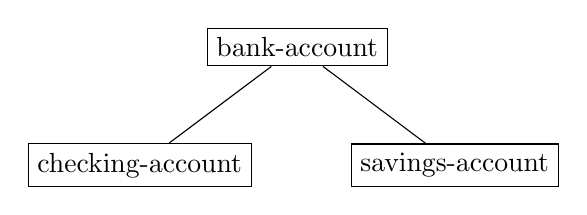
\begin{tikzpicture}[class/.style={draw},
                      sibling distance=4cm]
    \node [class] at (0,0) {bank-account}
      child { node [class] {checking-account} }
      child { node [class] {savings-account} };
  \end{tikzpicture}
  \caption{Иерархия классов}
\end{figure}

Основная форма \lstinline{DEFGENERIC} похожа на \lstinline{DEFUN}, за тем исключением, что нет тела функции. Список параметров \lstinline{DEFGENERIC} определяет параметры, которые должны приниматься всеми методами, определенными для данной обобщенной функции.
\begin{cllst}{}{}
(defgeneric withdraw (account amount)
    (:documentation "Withdraw the specified amount from the account.
  Signal an error if the current balance is less than amount."))
\end{cllst}

Методы реализуют поведение для определенных типов некоторых (или всех) параметров, определенных обобщенной функцией. Есть два метода специализации: по типу и по коокретному объекту (равенство проверяется с помощью \lstinline{EQL}).

Методы должны иметь то же самое количество обязательных и необязательных параметров и принимать любые аргументы, относящиеся к остаточным (\lstinline{&rest}) или именованным (\lstinline{&key}, \lstinline{&allow-other-keys}) параметрам, определенным в обобщенной функции. Метод также может указывать именованные параметры, не указанные в списке параметров обобщенной функции. Когда вызывается обобщенная функция, будет принят любой именованный параметр, указанный обобщенной функцией или любым другим подходящим методом.
\begin{cllst}{}{}
(defmethod withdraw ((account bank-account) amount)
    (when (< (balance account) amount)
      (error "Account overdrawn."))
    (decf (balance account) amount))
\end{cllst}

Функция \lstinline{CALL-NEXT-METHOD} является частью системы обобщенных функций и используется для комбинации подходящих методов. Она сообщает, что контроль должен быть передан от текущего метода, к методу, специализированному для \lstinline{bank-account}. Когда он вызывается без аргументов, следующий в цепочке метод будет вызван с теми же аргументами, которые были переданы обобщенной функции. Он также может быть вызван с явным указанием аргументов, которые будут переданы следующему методу.

\begin{cllst}{}{}
(defmethod withdraw ((account checking-account) amount)
  (let ((overdraft (- amount (balance account))))
    (when (plusp overdraft)
      (withdraw (overdraft-account account) overdraft)
      (incf (balance account) overdraft)))
  (call-next-method))
\end{cllst}

Форма, указанная в \lstinline{EQL}-специализаторе, который используется для указания объекта вычисляется один раз, когда вычисляется \lstinline{DEFMETHOD}.
\begin{cllst}{Пример EQL-специализатора}{}
(defmethod withdraw ((account (eql *account-of-bank-president*)) amount)
  (let ((overdraft (- amount (balance account))))
    (when (plusp overdraft)
      (incf (balance account) (embezzle *bank* overdraft)))
  (call-next-method)))
\end{cllst}

\subsection{Комбинирование методов}
Обобщенная функция при каждом запуске создают \emph{эффективный метод} из методов, для которых применимы текущие параметры. Эффективный метод строится в три этапа:
\begin{enumerate}
  \item Обобщенная функция строит список методов, которые применимы к переданным аргументам.
  \item Полученный список методов сортируется в соответствии со специализированными параметрами. При сортировке специализаторы сравниваются слева направо (порядок можно изменить с помощью \lstinline{:argument-precedence-order} в \lstinline{DEFGENERIC}). Первыми в списке  ставится метод с более специфичным специализатором.
  \item Методы по порядку берутся из списка и их код комбинируется, образуя эффективный метод.
\end{enumerate}

В типичном случае, если два специализатора класса отличаются, то один будет подклассом другого. В этом случае специализатор, именующий подкласс, считается более специфичным. Поэтому метод, который специализирован для счета с классом \lstinline{checking-account} будет рассматриваться как более специфичный, чем метод, специализированный для класса \lstinline{bank-account}.

\lstinline{EQL}-специализатор всегда более специфичен, чем любой специализатор класса. Если \lstinline{EQL}-специализатор конкретного параметра имеет более одного метода, то все они должны иметь одинаковые \lstinline{EQL}-специализаторы. Сравнение данных методов происходит на основе других параметров.

\subsubsection{Стандартный комбинатор методов}
Рассмотрим, как отсортированный список методов комбинируется в эффективный метод. По умолчанию обобщенные функции используют \emph{стандартный комбинатор методов}. Стандартный комбинатор объединяет методы таким образом, что сначала запускается наиболее специфичный метод, а каждый метод может передать управление следующему, используя \lstinline{CALL-NEXT-METHOD}.

До сих пор были рассмотрены только основные методы (в которых, как правило, реализуется основной функционал). Стандартный комбинатор методов также поддерживает три вида вспомогательных методов: \lstinline{:before}, \lstinline{:after} и \lstinline{:around}. Например:
\begin{cllst}{}{}
(defmethod withdraw :before ((account bank-account) amount) ...)
\end{cllst}

Каждый вид вспомогательных методов комбинируется в эффективный метод разными способами. Все применимые методы \lstinline{:before} (не только наиболее специфические) запускаются как часть эффективного метода. Они запускаются до наиболее специфического основного метода, начиная с самого специфического.
\begin{cllst}{}{}
(defmethod withdraw :before ((account checking-account) amount)
  (let ((overdraft (- amount (balance account))))
    (when (plusp overdraft)
      (withdraw (overdraft-account account) overdraft)
      (incf (balance account) overdraft))))
\end{cllst}

Все методы \lstinline{:after} запускаются после основного метода, начиная с наименее специфичного. Методы \lstinline{:around} запускается вместо других применимых методов, но внутри этого метода есть возможность вызвать любой другой метод.

Семантика стандартного комбинатора методов:
\begin{itemize}
  \item Если определёны \lstinline{:around} методы, то вызывается наиболее специфичный. Его результат будет результатом вызовы обобщённой функции.
  \item Внутри \lstinline{:around} метода можно использовать \lstinline{CALL-NEXT-METHOD}. Когда следующий метод завершается, можно выполнять дальше какой-либо код. Если используется \lstinline{CALL-NEXT-METHOD}, но нет применимого метода, то вызывается обобщённая функция \lstinline{NO-NEXT-METHOD}. Функция \lstinline{NEXT-METHOD-P} может быть использована для определения, есть ли следующий метод.
  \item Если в \lstinline{:around} вызывается \lstinline{CALL-NEXT-METHOD}, то следующий наиболее специфический \lstinline{:around} метод вызывается. Если нет следующего \lstinline{:around} метода или же был вызван наименее специфический \lstinline{:around} метод, то другие методы вызываются по следующим правилам:
    \begin{itemize}
      \item Вызываются все \lstinline{:before} методы, начиная с наиболее специфического. Их возвращаемые значения игнорируются. Является ошибкой вывоз \lstinline{CALL-NEXT-METHOD} из этих методов.
      \item Вызывается наиболее специфический основной метод. Внутри этого метод можно использовать \lstinline{CALL-NEXT-METHOD} для вызова следующего наиболее специфического основного метода. Когда следующий метод завершается, можно выполнять дальше какой-либо код. Если используется \lstinline{CALL-NEXT-METHOD}, но нет применимого основного метода, то вызывается обобщённая функция \lstinline{NO-NEXT-METHOD}. Функция \lstinline{NEXT-METHOD-P} может быть использована для определения, есть ли следующий метод. Если \lstinline{CALL-NEXT-METHOD} не используется в основном методе, то выполнение основных методов на нём и прекращается.
      \item Вызываются все \lstinline{:after} методы, начиная с наименее специфического. Их возвращаемые значения игнорируются. Является ошибкой вывоз \lstinline{CALL-NEXT-METHOD} из этих методов.
    \end{itemize}
  \item Если ни один \lstinline{:around} метод не был вызван, тогда результатом будет значение, возвращённое наиболее специфическим основным методом. \lstinline{CALL-NEXT-METHOD}, вызванный в наименее специфическом \lstinline{:around} методе, возвращает результат выполнения наиболее специфического основного метода.
\end{itemize}

При стандартном комбинаторе методов, является ошибкой вызывать обобщённую функцию с определёнными вспомогательными методами, но не определёнными основными.

\begin{cllst}{Иллюстрация порядка запуска основного и вспомогательных методов}{}
;;; integer => rational => real => number => t
(defgeneric speak (arg))

(defmethod speak ((arg number))
  (format t "number  : primary method~%"))

(defmethod speak ((arg integer))
  (format t "integer : primary method~%")
  (call-next-method))

(defmethod speak :before ((arg number))
  (format t "number  : before method~%"))

(defmethod speak :before ((arg integer))
  (format t "integer : before method~%"))

(defmethod speak :after ((arg number))
  (format t "number  : after method~%"))

(defmethod speak :after ((arg integer))
  (format t "integer : after method~%"))

(defmethod speak :around ((arg number))
  (format t "number  : around method~%")
  (call-next-method))

(defmethod speak :around ((arg integer))
  (format t "integer : around method~%")
  (call-next-method))

CL-USER> (speak 1)
integer : around method
number  : around method
integer : before method
number  : before method
integer : primary method
number  : primary method
number  : after method
integer : after method
NIL
\end{cllst}

\subsubsection{Другие комбинаторы методов}
CL в стандартной поставке имеет еще 9 других комбинаторов методов: \lstinline{+}, \lstinline{and}, \lstinline{append}, \lstinline{list}, \lstinline{max}, \lstinline{min}, \lstinline{nconc}, \lstinline{or} и \lstinline{progn}. Всё они ведут себя одинаковым образом: вместо вызова наиболее специфического метода, который в свою очередь может вызывать менее специфические, эти комбинаторы создают эффективный метод, который вычисляет все основные методы по порядку и передаёт результаты как аргументы функции с соответвующим именем комбинатора методов. Также эти комбинаторы поддерживают \lstinline{:around} методы.

Например, обобщённая функция, которая использует \lstinline{+} комбинатор, вернёт сумму всех значений, возвращённых основными методами. Следуем помнить, что при вызове обобщённой функции, которая использует \lstinline{and} или \lstinline{or} комбинатор, могут быть вычислены не все основные методы, если в вычислении конкретного метода нет необходимости.

По умолчанию, основные методы вычисляются, начиная с наиболее специфического. Можно изменить этот порядок на обратный, используя опцию \lstinline{:method-combination} в определении обобщённой функции.

\begin{cllst}{Пример использования простого комбинатора}{}
(defgeneric priority (job)
  (:documentation "Return the priority at which the job should be run.")
  (:method-combination + :most-specific-last))

(defmethod priority + ((job express-job)) 10)
\end{cllst}

Подытожим. Методы могут быть двух типов:
\begin{itemize}
  \item \lstinline{:around} методы. Являются тем же, что и \lstinline{:around} методы в стандартном комбинаторе методов. Поэтому в них можно использовать \lstinline{CALL-NEXT-METHOD} и \lstinline{NO-NEXT-METHOD-P}.
  \item Основные методы с таким же именем квалификатора, как и у соответсвующего комбинатора методов. Внутри этих методов нельзя вызывать \lstinline{CALL-NEXT-METHOD} и \lstinline{NO-NEXT-METHOD-P}.
\end{itemize}

Собственные комбинаторы методов можно определить, используя \lstinline{DEFINE-METHOD-COMBINATION}.
